\section{Auswertung}
\subsection{Zählrohr-Charakteristik}
In der Tabelle (\ref{tab:1}) sind die folgenden Messdaten aufgelistet und in
der Abbilung (\ref{abb:6}) graphisch dargestellt.
\begin{table}[H]
  \centering
  \caption{Messaufnahme zur Bestimmung des Plateaus.}
  \label{tab:1}
  \begin{tabular}{c c c c c c c c}
    \toprule
    $U \, /\, V$ & $N$ & $U \, /\, V$ & $N$ & $U \, /\, V$ & $N$ & $U \, /\, V$ &$N$ \\
    \midrule
\cellcolor{red}300 & \cellcolor{red}0 &410 & 13155 &530& 13336 &640& 13563\\
    310 & 12111 &420 & 13885 &540& 13225 &650& 13917\\
    320 & 12575 &430 & 12954 &550& 13318 &660& 13709\\
    330 & 12674 &450 & 13184 &560& 13376 &670& 13721\\
    340 & 12504 &460 & 13193 &570& 13200 &680& 13918\\
    350 & 12753 &470 & 13011 &580& 13514 &690& 13663\\
    360 & 12838 &480 & 13205 &590& 13438 &700& 14302\\
    370 & 12961 &490 & 13022 &600& 13363 &-& -\\
    380 & 12936 &500 & 13303 &610& 13288 &-& -\\
    390 & 12794 &510 & 13076 &620& 13446 &-& -\\
    400 & 13076 &520 & 13363 &630& 13495 &-& -\\
    \bottomrule
  \end{tabular}
\end{table}
\begin{figure}[H]
  \centering
  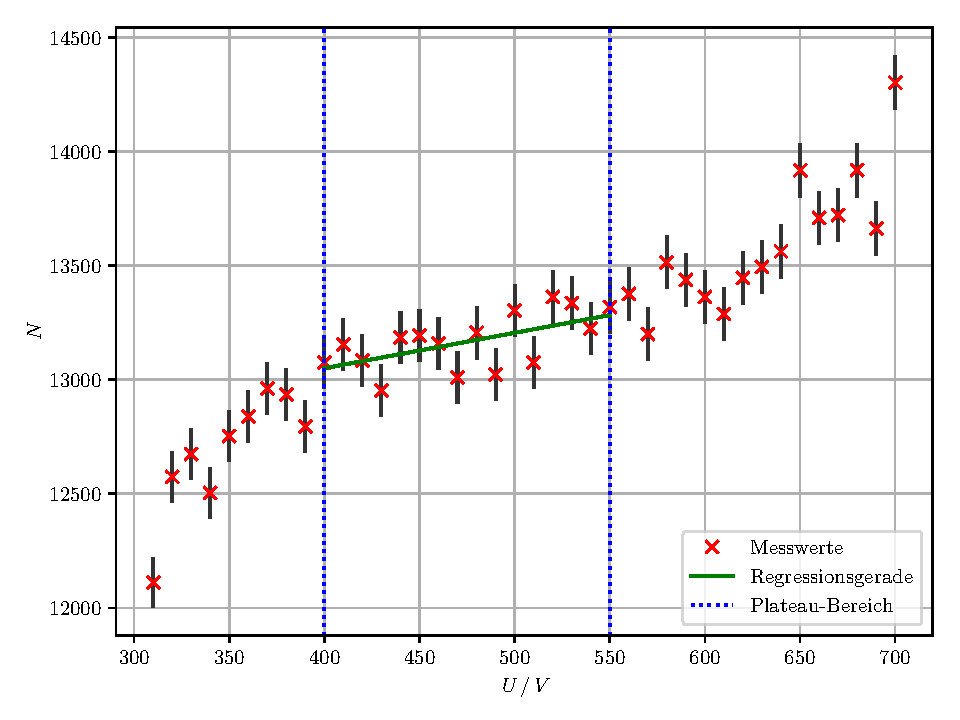
\includegraphics{plot1.pdf}
  \caption{Darstellung der Messdaten mit Fehlerbalken sowie die Einteilung des Plateaus.}
  \label{abb:6}
\end{figure}
Es ist zu beachten, dass der erste Messwert (rötlich hinterlegt) nicht in der Auswertung berücksichtig wird,
da sie physikalisch nicht sinnvoll ist.
Die Länge des Plateaus beginnt bei $\SI{400}{\volt}$ und endet bei $\SI{550}{\volt}$. Für diesen Kurvenabschnitt wird eine lineare Auschgleichsrechnung
\begin{align}
  y & = m \cdot x + b \label{eq:9}\\
  m & = \frac {\bar{xy} - \bar{x} \cdot \bar{y}} {\bar{x^2} -\bar{x}^2}&  \label{fel:1}\\
  b & = \frac {\bar{y} \cdot \bar{x}^2 - \bar{xy} \cdot \bar{x}} {\bar{x^2}-\bar{x}^2}& \label{fel:2}
\end{align}
durchgeführt.
Somit ergibt sich für die Parameter der Geraden:
\begin{itemize}
  \item m = \SI{1.55 \pm 0,55}{1\per\volt}
  \item b = 12429,16 \pm \, 264,59
\end{itemize}

Anschließend wird die Plateau-Steigerung in $\%$ pro $100 \, V$ mit
\begin{equation*}
  s = \frac{f(500)}{f(400)} \cdot 100 - 100 \%
\end{equation*}
bestimmt.
Die Steigerung beträgt $s = \SI{1.2 \pm 0.4}{\%\per\volt}$.
\subsection{Totzeit des Zählrohrs}
Wie in der Durchführung angesprochen wurde, wird zunächst die Totzeit sowie die Erhohlungszeit mit Hilfe des Oszilloskops
abgelesen. In der Tabelle (\ref{tab:2}) werden die Ablesungen dargestellt und anschließend wird der Mittelwert sowie die Standardabweichung
bestimmt.
\begin{table}[H]
  \centering
  \caption{Messdaten von der Ablesung am Oszilloskop.}
  \label{tab:2}
  \begin{tabular}{c c c}
    \toprule
    $U \, /\, V$ & $T_\text{tot} / s$ & $T_\text{re} / s$\\
    400 & 0.18 & 0.42\\
    500 & 0.2 & 0.7\\
    600 & 0.22 & 0.88\\
    \bottomrule
  \end{tabular}
\end{table}
Für den Mittelwert sowie die Standardabweichung werden die Formel (\ref{fel:3}) und (\ref{fel:4})
\begin{equation}
    \bar{x} = \frac{1}{N} \sum_{i=1}^{N} x_i
    \label{fel:3}
\end{equation}
\begin{equation}
  \Delta \bar{x} = \frac{1}{\sqrt{N}\sqrt{N-1}} \sqrt{\sum_{i}(x_i-\bar{x})^2}
  \label{fel:4}
\end{equation}
verwendet. Es folgt für die beiden Zeiten folgende Werte:
\begin{itemize}
  \item $T_\text{tot} = \SI{0,2 \pm 0,01}{\second}$
  \item $T_\text{re} = \SI{0,67 \pm 0,19}{\second}$
\end{itemize}
Nun wird die Totzeit mithilfe der Zwei-Quellen-Methode bestimmt.
Die Messaufnahmen für die beiden Präperate ergeben:
\begin{itemize}
  \item $N_1 = 13100$
  \item $N_2 = 1393$
  \item $N_{1+2} = 14668$
\end{itemize}
Zur Berechnung der Totzeit wird die Formel (\ref{eq:2}) verwendet.
Das Ergebnis  für die Totzeit lautet:
\begin{equation*}
  T_{Totzeit} = (-5 \pm 5) \cdot 10^{-6} \, s
\end{equation*}
Die Totzeit ist physikalisch nicht sinnvoll, da es keine negative Zeit gibt.
\subsection{Messung der freigesetzen Ladungsmengen}
Für die Berechnung der Ladungsmenge wird die Formel (\ref{eq:1}) umgestellt
\begin{equation*}
  \Delta Q =\underbrace{n}_{\mathclap{\text{Anzahl}}} \cdot \overbrace{e}^{\mathclap{\text{Elementarladung}}} = \frac{I \cdot \Delta t}{Z}
\end{equation*}
Da nur die Anzahl der Teilchen gesucht wird, wird die vorherige Gleichung noch durch die Elementarladung geteilt und in der Tabelle (\ref{tab:3})
dargestellt. Dabei ist Z fehlerbehaftet.
\begin{table}[H]
  \centering
  \caption{Messung bei $U=520 \, V$ und $\Delta t = 60 \, s$.}
  \label{tab:3}
      \begin{tabular}{c c c c c c c c c c c c}
        \toprule
        $U \, /\, V$ & $I \,/\, \mu A $ & $n \,/\, 10^{10} Teilchen$ &
        $U \, /\, V$ & $I \,/\, \mu A $ & $n \,/\, 10^{10} Teilchen$ &
        $U \, /\, V$ & $I \,/\, \mu A $ & $n \,/\, 10^{10} Teilchen$ &
        $U \, /\, V$ & $I \,/\, \mu A $ & $n \,/\, 10^{10} Teilchen$ \\
        \midrule
        310 & 0.1 & 0.309 \pm 0.002 & 410 & 0.3 & 0.855 \pm 0.007 & 510 & 0.6 & 1.721 \pm 0.015 & 610 & 0.9 & 2.539 \pm 0.022\\
        320 & 0.2 & 0.596 \pm 0.005 & 420 & 0.4 & 1.146 \pm 0.010 & 520 & 0.6 & 1.684 \pm 0.015 & 620 & 1.0 & 2.789 \pm 0.023\\
        330 & 0.2 & 0.591 \pm 0.005 & 430 & 0.4 & 1.158 \pm 0.010 & 530 & 0.7 & 1.968 \pm 0.017 & 630 & 1.0 & 2.779 \pm 0.024\\
        340 & 0.2 & 0.599 \pm 0.005 & 440 & 0.4 & 1.138 \pm 0.009 & 540 & 0.7 & 1.985 \pm 0.017 & 640 & 1.0 & 2.765 \pm 0.024\\
        350 & 0.2 & 0.588 \pm 0.005 & 450 & 0.5 & 1.421 \pm 0.012 & 550 & 0.8 & 2.253 \pm 0.020 & 650 & 1.0 & 2.695 \pm 0.023\\
        360 & 0.2 & 0.584 \pm 0.005 & 460 & 0.5 & 1.424 \pm 0.012 & 560 & 0.8 & 2.243 \pm 0.019 & 660 & 1.0 & 2.735 \pm 0.023\\
        370 & 0.2 & 0.579 \pm 0.005 & 470 & 0.5 & 1.441 \pm 0.013 & 570 & 0.8 & 2.273 \pm 0.020 & 670 & 1.1 & 3.006 \pm 0.026\\
        380 & 0.3 & 0.869 \pm 0.007 & 480 & 0.6 & 1.704 \pm 0.015 & 580 & 0.8 & 2.219 \pm 0.019 & 680 & 1.1 & 2.964 \pm 0.025\\
        390 & 0.3 & 0.879 \pm 0.008 & 490 & 0.6 & 1.728 \pm 0.015 & 590 & 0.8 & 2.232 \pm 0.019 & 690 & 1.2 & 3.294 \pm 0.028\\
        400 & 0.3 & 0.860 \pm 0.008 & 500 & 0.6 & 1.691 \pm 0.014 & 600 & 0.9 & 2.526 \pm 0.022 & 700 & 1.3 & 3.409 \pm 0.029\\
        \bottomrule
      \end{tabular}
    \end{table}
